\documentclass{article}

\usepackage{pdfpages}
\usepackage{mathtools}

\author{Daniel Fernandes \and Yue Li}
\title{ECE 110 Final Design Project}
\date{December 6, 2012}

\begin{document}
\maketitle

\part{Introduction}
The final design project involves programming a small, two-motor car to follow a white line around a track using only IR Sensors combined with either TTL Logic or an Arduino microprocessor. We have chosen an Arduino Micro, with a CAB Module (H-Bridge) and Arduino-compatible CA module (BJT Transistor) for each side of the car.
\part{Design}
\section{Hardware Design}
\subsection{Sensors}
Our sensor layout uses two IR sensors (A5 and A6) in the outermost bar to detect splits and for stop detection. When both sensors see the white line, this indicates that we have reached a split. After two splits, we reuse this circuit for stop detection.\\
The second sensor bar, placed closer to the car, uses two IR sensors (A9 and A10) on the outer edges for right turn detection. Five more sensors (A0-A4) are distributed symmetrically about the center axis of the sensor bar. The center sensor (A2) is critical for detecting the color for split detection. The two sensors adjacent from the center (A1 \& A3) are used for the Tape Avoiding / Tape Seeking navigation scheme. The remaining two sensors (A0 \& A4) are used for right turn detection. They were initially placed for a PID loop, but the PID loop was not suited to our needs.
\subsection{CAB}
The CAB module provides a H-Bridge in order to invert motor direction with a single digital output. The key to making the CAB module work is to connect Vmotor and GND for the Vmotor pin to the Motor1 and Motor2 pins of the CA Module. This allows us to control the current through the CAB from the CA.\\
In order to control the polarity of the H-Bridge, we shorted pins T2 and T4 to ground, connected T1 to a digital output pin from the Arduino and used a NOT TTL chip to invert the signal from T1 to T3.
\subsection{CA Module}
The Arduino CA module was straightforward to setup. The Motor1 and Motor2 pins could go directly to the leads for the motor, but we decided to run these through the CAB H-Bridge for more functionality. The ON/OFF pin of the CA Module is connected to a PWM output pin on the Arduino.
\subsection{Arduino}
We initially started with a standard Arduino UNO available from the ECE Store, but we found the Arduino Micro (from AdaFruit Industries) to offer better functionality in a better form factor. The Arduino Micro has all the pins of a Arduino UNO, but uses an smaller SMD (surface mount device) chip rather the DIP (dual in-line package) chip used in the UNO. It also has headers that make it a drop-in solution for a protoboard like the one used in the ECE 110 lab. In fact, the Micro has more analog inputs available than the UNO which was useful for our design.
\subsection{Wiring}
Our wiring used the two innermost power rails to provide 5V to logic chips and the two outermost power rails to provide 12V to the motors. We rewired the board several times, using the shortest wires possible to minimize clutter. IR Sensor inputs were routed out from the Arduino to the front of the vehicle, making the setup of the analog sensor bar a less arduous task.
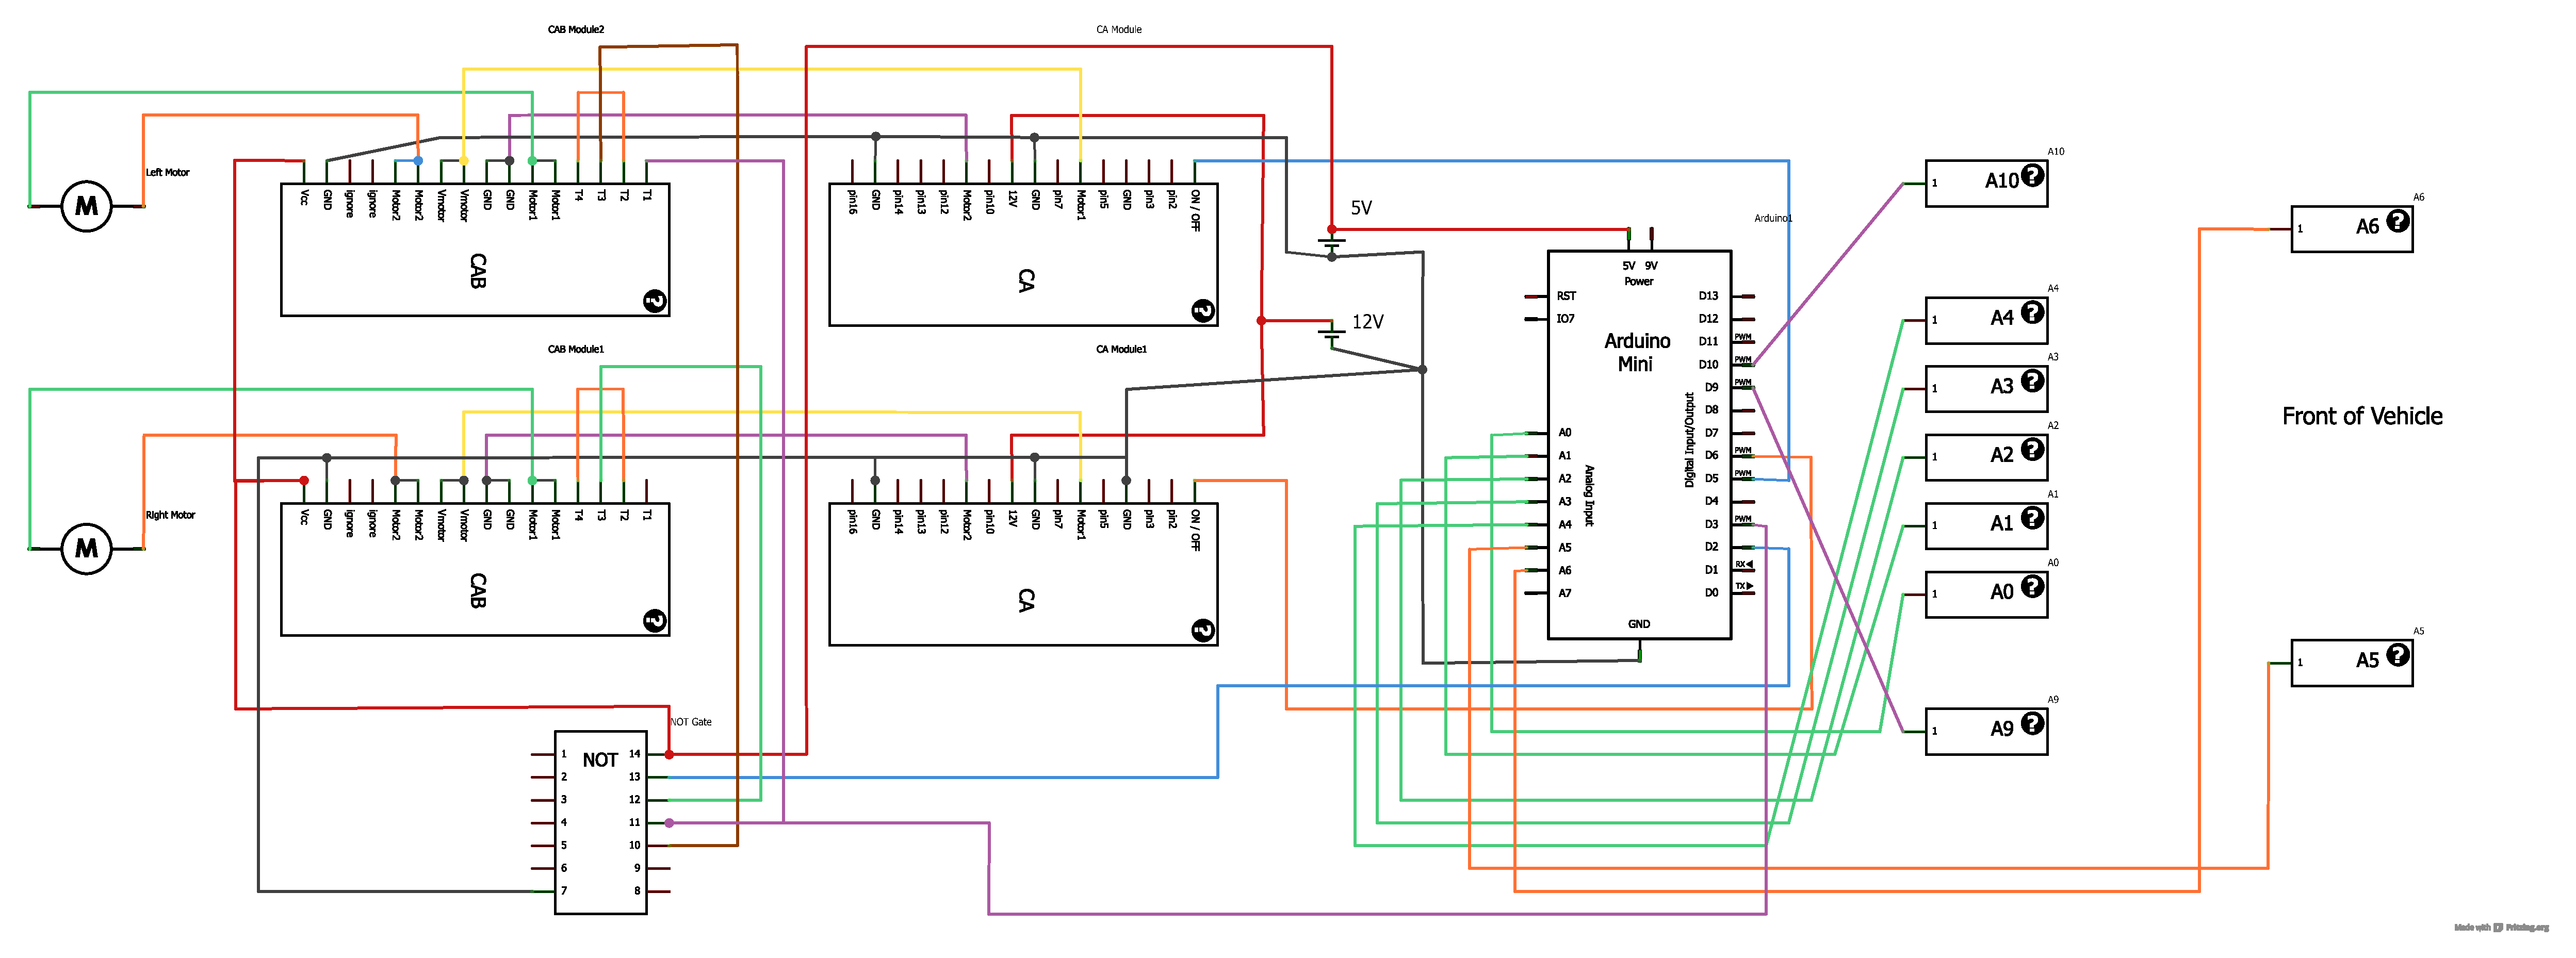
\includepdf[angle=90]{ece110sketch_schem.pdf}
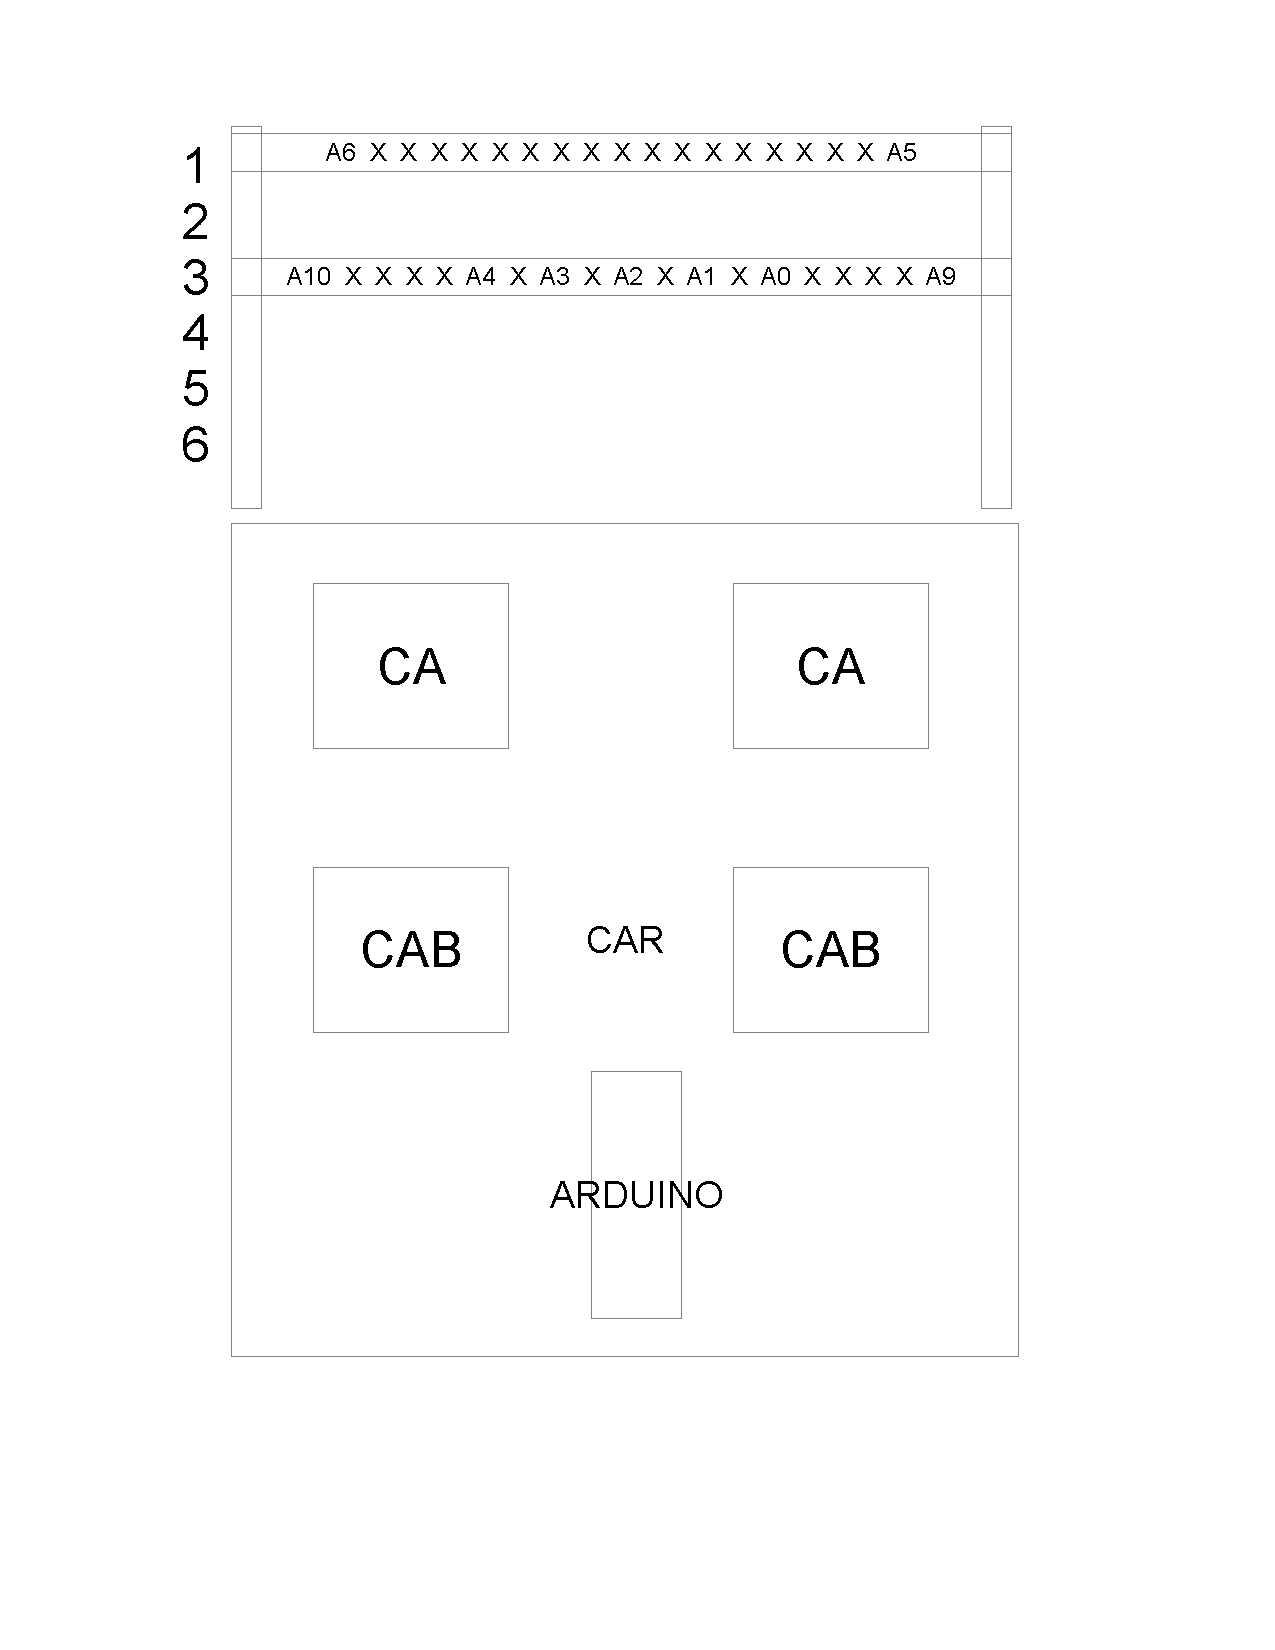
\includepdf{ece110drawings.pdf}
\section{Software Design}
\subsection{Calibration Code}
Rather than using a comparator circuit, we took advantage of the Arduino Micro's massive 1KB EEPROM storage to store sensor values. These sampled values were used to computed a "white threshold" and "black threshold". The white threshold being the lowest value before a sensor could be declared white, and the black threshold indicating the highest value a sensor value could hold before it could no longer be declared black. Grey is between the black and white thresholds. To do this, we created a separate calibration program that asks the user over serial input what sensor is being calibrated and for what color (white or black). The program will print out the current values that sensor is reading and will save the last value received into the EEPROM once the user presses 'k'. The threshold values were computed using the following formulas:
\begin{align}
midpoint = \frac{whiteSample + blackSample}{2}\\
whiteThreshold = \frac{midpoint + whiteSample}{2}\\
blackThreshold = \frac{midpoint + blackSample}{2}
\end{align}
\subsection{PID Loop}
Initially, we tried using a PID Loop (Proportional-Integral-Derivative), but this did not pan out for several reasons. In a nutshell, the PID Loop is a type of feedback loop used that takes an input of error and outputs power to correct the error. The ``Proportional" part of the loop responds to immediate error, the ``Integral" part responds to past error, and the ``Derivative" part responds to future error. The PID Loop requires careful analysis to avoid problems such as ``Integral Windup" where too much error has been accumulated for too long and the output becomes too skewed. Another problem was trying to determine a numerical value for the error distribution. An effort was made towards this in the \textit{errorScore()} function but the benefits of such a complex system were not enough to justify the time investment for the limited lab sessions available.
\subsection{Tape Avoider / Tape Seeking Hybrid}
Once the PID plan had been abandoned, we chose one of the navigation schematics introduced in previous labs. This is essentially a Tape Avoiding circuit, except one side of the car always has a bit more power than the other. This forces the car to drive into the white line and recorrect itself. This gives the speed benefits of a Tape Avoiding circuit, with the accuracy advantages of a Tape Seeking circuit. This ended up being the design we chose for the final trial and it preformed exceptionally well. 
\subsection{Right Angle Turn Detection}
For right angle turn detection we test if a outermost sensor on the second sensor bar sees white (Sensors A9 \& A10), and another inner sensor on the same side sees white. The reason we need a second sensor is to ensure that we are actually at right turn and not crossing a split. For example, when the car turns right on a Y, the leftmost sensor would see white for a moment, which would incorrectly trigger the turning code.\\
Once we detect a turn, we drive forward a little bit, and start turning until the center sensor sees the line again.
\subsection{Split Detection}
The split detection occurs when the two frontmost sensors see white (Sensors A5 \& A6). The sensors are placed such that they trigger right when the centermost sensor (A2) is in an optimal position to read the color of the split. We use the color calibration mentioned previously to read if the center sensor sees grey or white. We act on this information by supplying turning power in the corresponding direction.
\subsection{Stop Detection}
After incurring two splits, we reuse the split detection sensors for stop detection and cut power to the motors.
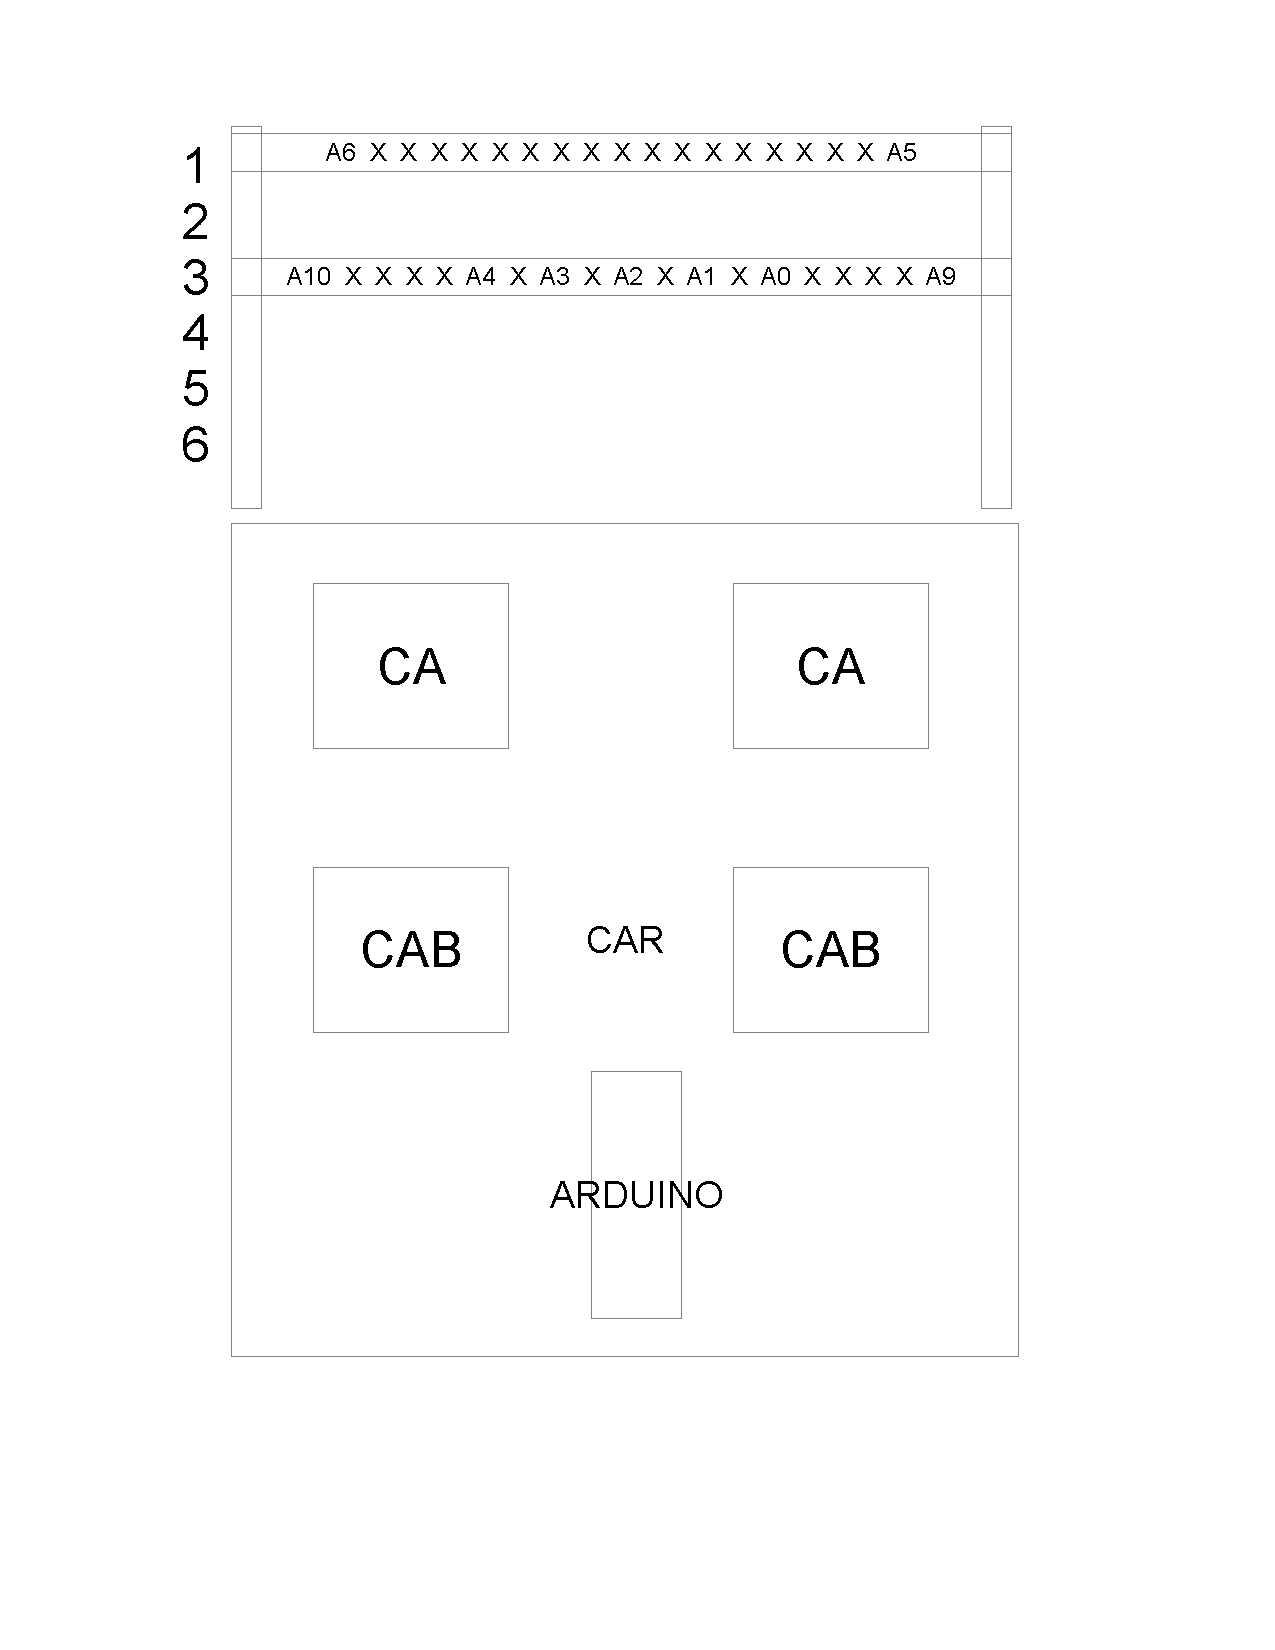
\includepdf[page=2]{ece110drawings.pdf}
\part{Design Philosophy}
Our design process started with the choice to use the Arduino microcontroller, rather than TTL logic. Using a microprocessor allows the design to use the same IR sensors for triggering different reactions. Many TTL logic designs have IR sensors dedicated to one task---such as split detection or stop detection. A microprocessor can address each IR sensor individually and use the same sensors for split detection and stop detection.\\
Additionally we put numerous debugging statements in the code that will printout the current state of the robot over the Arduino's USB interface. By reading this data, we were able to isolate and solve both hardware and software issues.
\part{Performance}
Our tape seeking / tape avoiding hybrid preformed excellently on the straight, curvy, and zig-zag parts of the track. The right turn detection circuit preformed much better than expected, the car would drive into the turn, backup and run into the turn again at a steeper angle, repeating the process until completed. Our split detection software successfully detected the first grey split, but incorrectly interpreted a white split, and went left. This was because our sensor bar was too close to the table, making grey and white indistinguishable. After moving the sensor bar up, we recalibrated all the sensors and showed the split detection correctly detected the color of the split, but the battery was too low and the time too little to try another attempt. We did not get to the point where we tested the stop detection. In the end we earned 35/40 points.

\part{Future Improvements}
In the future, we would like to add an LCD display to improve debugging efficiency. We would also add another IR sensor to the outermost sensor bar, in the centermost position for stop detection. Rather than counting the number of splits, which can be inaccurate, we can simply stop the car if all three sensors on the outermost bar return white. A true split would only trigger the two outermost sensors. For software, we would like to fully implement the PID loop.
\end{document}